\documentclass[12pt]{article}

\usepackage[english,spanish]{babel}
\usepackage[utf8]{inputenc} 
\usepackage{cite}
\usepackage{array}
\usepackage{enumerate}
\usepackage{multicol}
\usepackage{stix}
\usepackage{graphicx}
\usepackage{ragged2e}
\usepackage[a4paper,top=3cm,bottom=2cm,left=3cm,right=3cm,marginparwidth=1.75cm]{geometry}
\usepackage{amsmath}
\usepackage[colorinlistoftodos]{todonotes}
\usepackage[colorlinks=true, allcolors=blue]{hyperref}
\usepackage{mathpazo}

\begin{document}

\begin{titlepage}
	\newcommand{\HRule}{\rule{\linewidth}{0.5mm}} 
	
	\center 
	
	
	
	\textsc{\LARGE Instituto Tecnológico de Morelia }\\[1.5cm] 
    
    
\includegraphics[width=0.2\textwidth]{descarga.jpg}\\[1cm] 
	
	\textsc{\Large Ing. en Sistemas Computacionales}\\[0.5cm] 
	
	\textsc{\large Ensayo }\\[0.5cm] 
	
	
	
	\HRule\\[0.4cm]
	
	{\huge\bfseries Alfiles}\\[0.4cm]
	
	\HRule\\[0.6cm]
	
	\textsc{\large Inteligencia Artificial }\\[0.5cm]
	
	\begin{minipage}{0.4\textwidth}
		\begin{flushleft}
			\large
			\textit{Autor}\\
		    \textsc{David Zavala Moreno} 
		\end{flushleft}
	\end{minipage}
	~
	\begin{minipage}{0.5\textwidth}
		\begin{flushright}
			\large
			\textit{Profesor}\\
			\textsc{J. Eduardo Alcaraz Chávez}
		\end{flushright}
	\end{minipage}
  
\end{titlepage}

\newpage
\newpage
\tableofcontents 
\newpage

\section{Introducción}

En el mundo del ajedrez existen muchos problemas, acertijos y conjeturas sobre los movimientos y espacios dentro del tablero de juego. Henry Ernest Dudeney fue el mayor creador de rompecabezas y acertijos matemáticos británico. Sin ninguna formación reglada en el área de las matemáticas sus ideas y aportaciones fueron reconocidas por la oficialidad matemática, entre sus mas importantes aportes se encuentran:
\begin{itemize}
    \item Deserciones geométricas
    \item Cuadrados mágicos 
\end{itemize}

En este breve ensayo nos centraremos en un problema de ajedrez que creó, el cual consiste en la siguiente imagen del tablero recortado como base.

\begin{figure}[h]
\centering
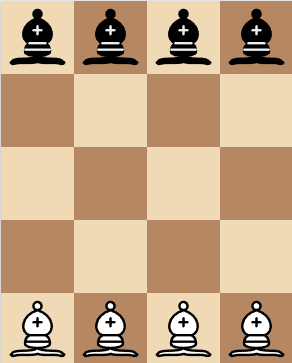
\includegraphics[width=0.4\textwidth]{1.png}
\caption{\label{fig:xx}Caso base del problema de los alfiles.}
\end{figure}

El problema consiste en colocar ocho alfiles (cuatro negros y cuatro blancos) en el tablero de ajedrez reducido (5 filas por 4 columnas). Lo que se tiene que hacer es que los alfiles negros intercambien sus posiciones con los blancos, ningún alfil debe atacar en ningún momento otro del color opuesto.
Se deben alternar los movimientos, primero uno blanco, luego uno negro, luego uno blanco y así sucesivamente.

\section{Análisis de la solución}

Analizando mediante introspección el siguiente problema basando el método de solución por medio de fuerza bruta podemos observar la complejidad de este problema radica en el hecho de que los alfiles de colores opuestos no se ataquen entre ellos, ya que si fuera solo cambiarlos de posición no sería tan complicado.\\

Después de un largo análisis nos percatamos que el primer movimiento debe ser simétrico (mover las mismas piezas) entre ambos colores de alfiles. Al seguir intentando mover las piezas tratando de que no se atacarán entre si los alfiles, pudimos percatarnos de que a través de la simetría se puede resolver este problema.\\

Aunque después de tomar esta teoría como valida, se redujo la dificultad del problema en un cincuenta por ciento, se seguía teniendo un nivel de complejidad bastante alto ya que eran muchas las posibles combinaciones de movimientos que se podían hacer, después de muchos intentos se logro resolver este problema con 18 movimientos de capa color, los cuales son los siguientes: 

\begin{multicols}{2}
\begin{enumerate}
    \item B(17-14) N(2-5)
    \item B(16-7) N(3-12)
    \item B(18-13) N(1-6)
    \item B(14-4) N(5-15)
    \item B(7-2) N(12-17)
    \item B(13-8) N(6-11)
    \item B(4-9) N(15-10)
    \item B(8-18) N(11-1)
    \item B(9-3) N(10-6)
    \item B(19-9) N(0-10)
    \item B(2-8) N(17-11)
    \item B(9-12) N(10-7)
    \item B(18-15) N(1-4)
    \item B(15-0) N(4-19)
    \item B(8-5) N(11-14)
    \item B(12-6) N(7-13)
    \item B(5-2) N(14-17)
    \item B(6-1) N(13-18)
\end{enumerate}
\end{multicols}

\begin{figure}[h]
\centering
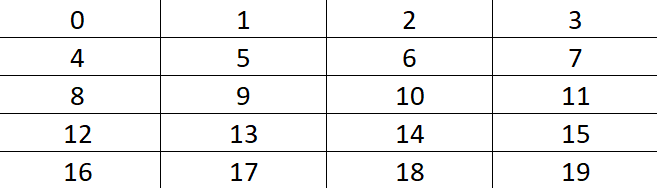
\includegraphics[width=0.8\textwidth]{2.png}
\caption{\label{fig:xx}Matriz del tablero.}
\end{figure}


\section{Conclusiones}

Se puede concluir de este ejercicio que se necesitan realizar movimientos simétricos entre ambos turnos, en este caso se logro resolver en dieciocho pares de movimientos, es posible definir un algoritmo capaz de resolver este problema, aún no se tiene establecido claramente uno pero por medio de condiciones anidadas se pueda resolver este problema.

\end{document}